\subsubsection{Samarbeidsindikator}

Det gir tre samarbeidsindikatorer, der man skal kunne se tendenser til utvikling av kommunikasjon i gruppen.
En rekke sosiale kvaliteter særpreger effektivt gruppesamarbeid \cite{orgorg}:

\begin{itemize}
	\item åpen kommunikasjon
	\item gjensidig tillit
	\item sosial støtte
	\item utnyttelse av individuelle forskjeller
\end{itemize}
	
Alle disse punktene kan kommenteres i forbindelse med gruppens sosiale utvikling.
Enighet om mål, og hvordan disse skulle oppnås, ble tidlig etablert i form av samarbeidskontrakten.
Ønsket om karakteren A har preget gruppens innsats, og fastsatte regler om oppmøte og leveringsfrister har fremmet profesjonalitet innad i gruppen.

\begin{figure}[h!]
	\begin{center}
		\caption{Gruppens første samarbeidsindikator.}
		\label{fig:samarbeidsindikator}
		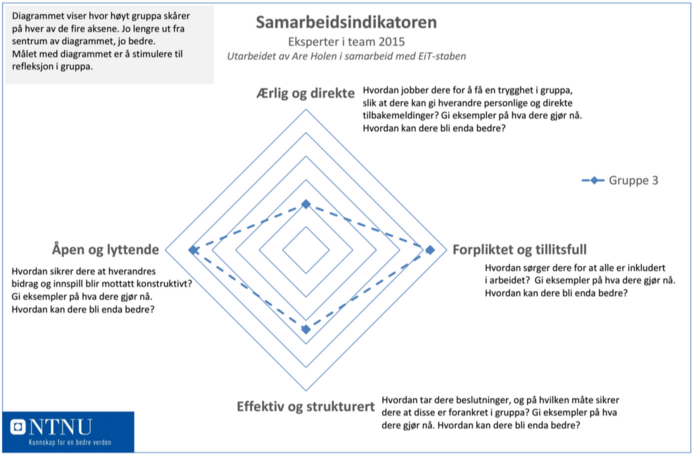
\includegraphics[width=0.9\textwidth]{samarbeidsindikator1.png}
	\end{center}
\end{figure}

\paragraph{Sosiale inntrykk}

En god sosial kommunikasjon og en god tone i gruppen hjelper til for å skape et positiv og trygt arbeidsmiljø.
Det gir medlemmer mer lyst til å samarbeide, og de føler seg mer komfortable med å jobbe sammen.
Et godt sosialt miljø i gruppen gjorde at medlemmene ble mer klare over hvilke personlighetstyper som fins i gruppen, noe som er svært viktig informasjon i et samarbeid.
Fra begynnelsen av prossessen har hvert enkelt gruppemedlem vært inkluderende og dedikert. 
Derfor ble, for eksempel, innsjekk og utsjekk alltid tatt på alvor.
I disse samlingene har individer fått mulighet til å vise tillit til hverandre og inkludere resten av gruppen i sitt liv. 
Det ble etterhvert en slags tradisjon, hvor vi følger hverandres prosjekt og ikke minst utvikling i andre området av livet.
Crossfit, barn, maraton, røyking, Bahamas, mat og Samfundet er noen temaer som har vært gjennomgått.

At gruppen har hatt så vennlig sosial kontakt medfører til både positive og negative konsekvenser.
Det positive er at samtlige gruppenmedlemmer ble motivert fra begynnelsen til å delta og gjøre en god innsats.
Ikke minst var det viktig for å bevare den gode tonen samt unngå eventuelle konflikter.

Kanskje er det dette fenomenet samarbeidsindikatoren adresserer når den viser at gruppen av vært lite ærlig og direkte.
Den gode tonen gjorde også at gruppen i begynnelsen har slitt noe med tid og struktur og tapte derfor på effektivitet.

Stemningen i gruppen har stort sett vært avslappet med tendenser til vitsing.
Det ble raskt tendenser til distraksjoner under gruppemøter, og behovet for å kalle til ro dukket opp ved flere anledninger, noe som førte til at gruppen innførte ordstyrer.

Det er ingen tvil om at sosialt god kommunikasjon går hånd i hånd med hvordan medlemmer jobber.
Siden alle har vært svært dediktert i arbeidet sitt og etterhvert fått tillit fra gruppen, fikk gruppen sigende et mer avslappende forhold til forsinkelser, fravær og fristforsinkelser.

Medlemmenes inkludering av hverandre og positive forhold til faget gjorde at medlemmene følte eierskap og ansvar i samarbeidet.
Samtlige medlemmer ble sett og hørt, og ingen fikk mulighet til å melde seg ut.
Gruppen har for eksempel bestemt seg for å dra på restaurant for å ferie sammen når rapportene er leverte. 
Det gjør at medlemmene er knyttet sammen og deler ansvar.
Å fokusere på at alt skulle gjøres sammen i sosial sammenheng har hatt positiv konsekvens i det faglige arbeidet.
\iffalse
(Eksempel av Jonas i konferans [forelesningen?] som satt alene, Karsten og Anna gjorde plass sånn at de kunne alle 3 sitte sammen, Crossfit dag, vi slette å ta ut en medlem av gruppe )


<Kort beskrivelse av den sosiale atmosfæren: Avslappet, tendens til vitsing, tendens til distractions under gruppemøter, tendens til å kalle til fokus når det trengs>
etc
Spørsmål:
Har vi hatt positiv innflytelse av at alle var villige til å gjøre en grundig jobb (gå etter A’en, samarbeidskontrakten)?
Var alle det fra start av, eller kom viljen til å gjøre en grundig jobb som følge av god teamfølelse?
“Veldig avslappet” pros and cons
Pros: Har dette gjort at folk ikke blir arrige over forseintkomminger og fristoverskridelser, i og med at alle på teamet føler seg trygge på at en innsatts blir gjort? 
Pros: Har dette gjort det lettere å håndtere uenigheter, siden folk har hatt god vilje og “likt” hverandre?
Har det vært nyttig som ‘sosial judo’ i å kunne snakke om konflikter i tidlig fase, lenge før kokepunkt?
Cons: Har det kostet oss verdiful tid, spesielt i den første halvdelen av faget? Var progresjon i arbeidet jevnlig handicappet? Gikk det ofte veldig sakte fremover? Brukte gruppen mye tid på unødvendig sosial prat? Kunne dette føre til frustrasjon blandt noen medlemmer på gruppen, og mindre hos andre, derved skape mulighet for konflikt (noen jobber hardt, andre prater bare tull)
Innflytelse av god sosial stemning på innsjekk/utsjekk: bryr folk seg om hverandre (referer til fagets beskrivelse av forskjellige team-egenskaper). F eks teamet bryr seg om de individuelle og hvilken overføringsverdi dette har til arbeidet.
 Anna røykestopp/maraton, Simen + sønn Odin, Ingelin CF progresjon, Martin mat (:))) /DJing/tech ansvar på singsaker studenthjem), Karsten mountainbike/Bahamastur, Jonas sine eventyr på samfundet 

<mangler spesifikke referanser til referat; vi må få samlet disse et sted>

\fi
